In the seminal paper by Einstein \cite{einsteinUberErzeugungUnd1905}, that laid foundations to Quantum Mechanics, Einstein postulated that light is made of discrete quanta of energy $E = h\nu$ to explain the observations by Hertz and J.J. Thompson; explaining the photoelectric effect. The effect can be described by the Equation \ref{eq:photoelectric} where $E_e$ the emitted kinetic energy, $h$ is the plank's constant, $\nu$ the frequency of the incoming photon and  $\phi$ the material-specific work function (also known as binding energy). 

\begin{equation}\label{eq:photoelectric}
    E_e = h\nu - \phi
\end{equation}

The equation describes how incident photons on a surface eject photoelectrons, provided the photon energy $h\nu$ exceeds $\phi$. This also highlights that the emitted kinetic energy $E_e$ does not depend on the photon flux (photon counts per second). However, the flux increases the total amount of electrons released from the material.

It is then apparent that the binding energy of electrons can be found by irradiating light onto the material and measuring the $E_e$ of photoelectrons. \gls{PES}, is exactly such a technique that leverages this principle to probe the electronic structure of materials. While the above equation describes at what energies electron come out, it does not explain why 



A complete treatment of photoemission process needs the quantum theory of light-matter interaction. However, many of the results can be explained by semi-classical theory\footnote{Semi-classical theory treats the light as a classical wave and the electrons as quantum particles.}.

TODO: Add more details about the photoelectric effect and the photoemission process.
% \section{Light-Matter Interaction}\label{section:light-matter-interaction}
% Where a complete description is not always necessary.

A variety of photoemission spectrometers can be devised depending on which parameters are varied and what is measured. Naturally, the most basic setup would measure the energy of the emitted electron as described in equation \ref{eq:photoelectric}, but it is also common to measure the surface parallel momentum ($k_x$, $k_y$)


the whole process of excitation, transport, and emission is treated as a single coherent process using the formalism of quantum mechanics. This approach incorporates the electronic structure, electron-electron interactions, and the surface barrier in a unified way, and describes the photoemission intensity  I(E, $k_x$, $k_y$)  as:


\section{Light Sources}\label{section:light-sources}
To perform \gls{PES}, it is imperative to first look at what the source of the electromagnetic radiation is necessary. The source needs to be monochromatic\footnote{Truly monochromatic radiation is physically impossible, and generally a range is considered.} and tunable, so that the only specific electrons are excited, allowing for precise measurement. Many materials of interest have binding energies lying in the UV to X-ray range. To measure not only the electronic states but also their dynamics, it becomes necessary to have a temporally coherent source.


\subsection{Laser}
The most ubiquitous of light sources--the laser--revolutionized experimental science as it enabled a vast range of phenomena to be precisely tested and observed, due to its high spatial and temporal coherence properties. A laser produces its light through a process known as stimulated emission, a process in which electrons, excited to higher energy states by an external energy source, emit photons as they return to lower energy states. These emitted photons, in turn, stimulate other electrons to release additional photons, leading to a cascade of coherent light. A process known as \gls{HHG} is used to generate ultrafast light of higher energies so that core electrons can be probed.  

\subsection{Synchrotron}
Particle accelerators, initially used for high energy physics experiments, which produce radiation as a byproduct of particles accelerating, found their use in spectroscopy. Soon, dedicated facilities providing extremely bright and tunable source of electromagnetic radiation emerged. One class of such facilities are known as Synchrotrons, which are named due to their cyclic design. Typically, bunches of electrons are accelerated by bending magnets, known as \glspl{undulator}, placed around a storage ring. These electrons are accelerated till they reach appropriate energies and provide a continuous source of radiation. Tangent to the ring, at certain points in the facility are beamlines which direct the radiation to the experimental end-stations, used to perform experiments in fields of life science, material science, and medicine to name a few.

There are several synchrotron facilities around the world, and in Germany such as BESSY II in Berlin, PETRA III at DESY campus in Hamburg.

\subsection{Free-Electron Laser}
TODO: Add more details about FELs
While Synchrotrons are excellent sources of light for a multitude of experiments, they have limitations in terms of the temporal coherence of the light produced. \glspl{FEL} are a class of light sources that overcome this limitation. \glspl{FEL} are linear particle accelerators that produce radiation through spontaneous emission (see \cite[Chapters 5 and 10]{foxQuantumOpticsIntroduction2006} for a detailed explanation of spontaneous emission).

Unlike traditional lasers, \glspl{FEL} do not require a traditional optical cavity or gain medium. Instead, they use a linear particle accelerator to produce a bunched electron beam, which is then passed through an undulator. The undulator is a series of magnets that produce a periodic magnetic field, causing the electrons to oscillate and emit radiation. The emitted radiation interacts with the electrons, leading to microbunching, which produces coherent radiation.

The light produced is of high peak brightness and can be compressed to femtosecond pulse durations, making it an ideal source for studying ultrafast phenomena.

An example scheme of the acceleration modules can be seen in Figure \ref{fig:flash-schematic}.

\begin{figure}
    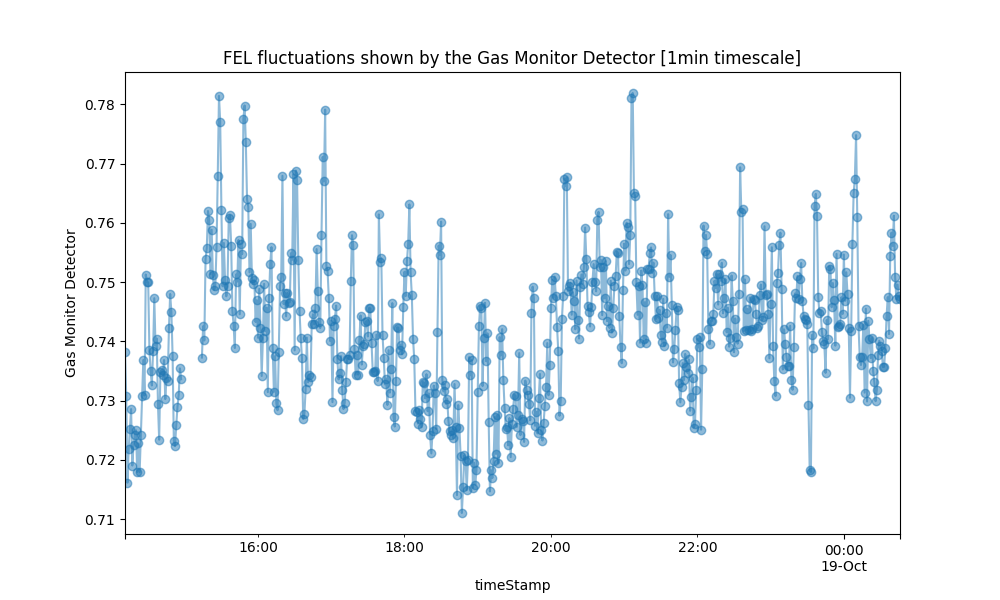
\includegraphics[width=1\linewidth]{images/2024-08-16-13-56-32.png}
\end{figure}


\section{HEXTOF instrument at FLASH}

\begin{figure}
    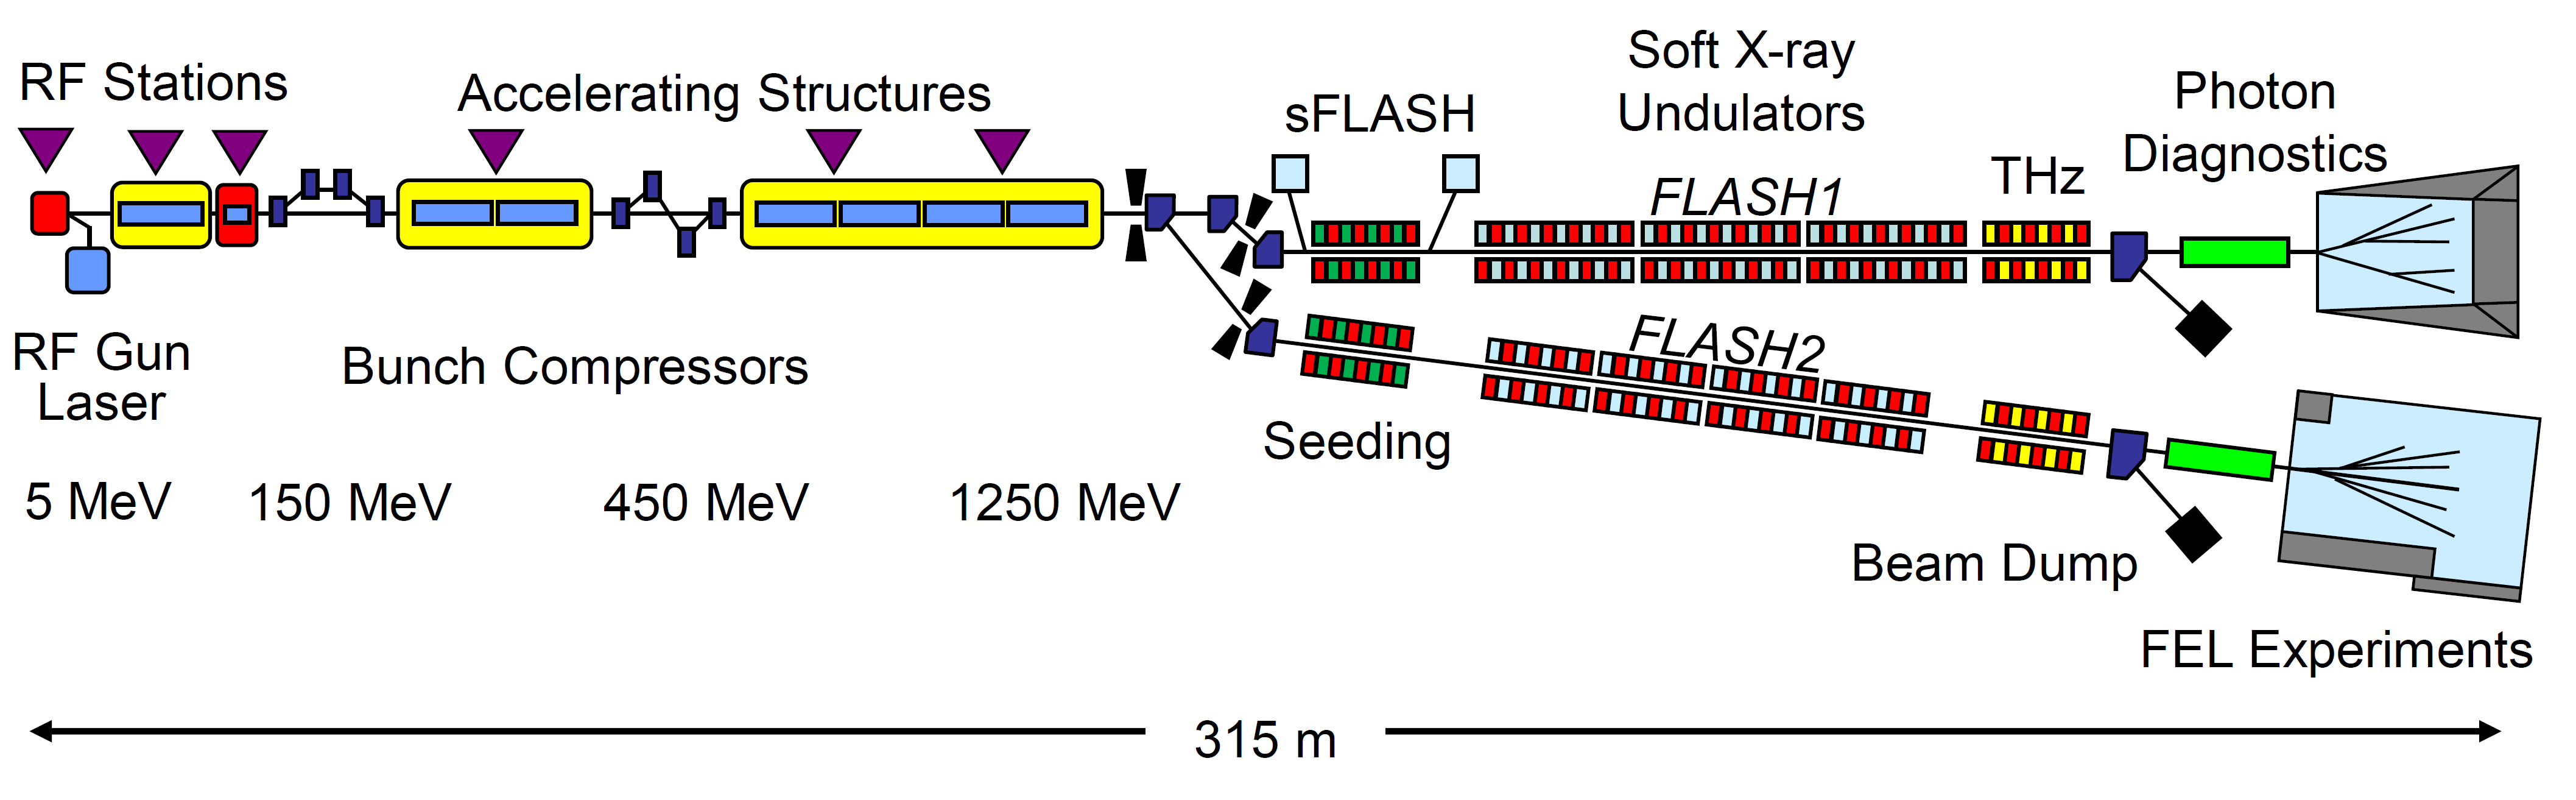
\includegraphics[width=1\linewidth]{images/flash_fel.png}
    \caption{Schematic view of \gls{FLASH} taken from \cite{faatzSimultaneousOperationTwo2016}.}
    \label{fig:flash-schematic}
\end{figure}

\gls{DESY} is a national research center in Germany that operates the \gls{FEL} \gls{FLASH} facility \cite{ackermannOperationFreeelectronLaser2007,tiedtkeSoftXrayFreeelectron2009} that produces ultrashort \gls{XUV} and soft X-ray radiation in the wavelength range of \qtyrange{4}{50}{\nm} in the fundamental, and as low as \qty{1.7}{\nm} in the third harmonic, corresponding to a total photon energy range of \qtyrange{25}{830}{\eV}. With an average pulse energy of \qtyrange{1}{500}{\micro\joule}, and pulse durations \qty{<10}{\fs}, peak powers of \qtyrange{1}{5}{\giga\watt} can be reached. This makes it an ideal source for studying ultrafast processes in materials and molecules.   

The \gls{HEXTOF} instrument, comissoned at \gls{FLASH}

One of the standout features of HEXTOF is its multidimensional recording scheme. This approach allows for simultaneous measurement of multiple parameters, including momentum (k-space) and time (t), resulting in a three-dimensional (3D) dataset. The ability to resolve kx, ky, and time enables researchers to capture dynamic processes in materials, such as ultrafast electron dynamics and structural changes, with unprecedented detail.

The 3D data acquisition is facilitated by a \gls{DLD}, which provides high spatial and temporal resolution. This capability is particularly advantageous for studying materials with complex electronic structures, as it allows for the exploration of both surface and bulk phenomena by tuning the probing depth through the kinetic energy of emitted photoelectrons 

% I(E, k_x, k_y) \propto |\langle \psi_f | \mathbf{A} \cdot \mathbf{p} | \psi_i \rangle|^2 \delta(E - E_f)

% where:

% 	•	 \psi_i  and  \psi_f  are the initial and final electron wavefunctions.
% 	•	 \mathbf{A} \cdot \mathbf{p}  is the interaction term representing the coupling between the electron and the incident photon (with vector potential  \mathbf{A}  and momentum operator  \mathbf{p} ).
% 	•	The delta function  \delta(E - E_f)  ensures energy conservation.


The \gls{HEXTOF} instrument is capable of performing time- and momentum-resolved photoemission studies 
\begin{figure}
    \centering
    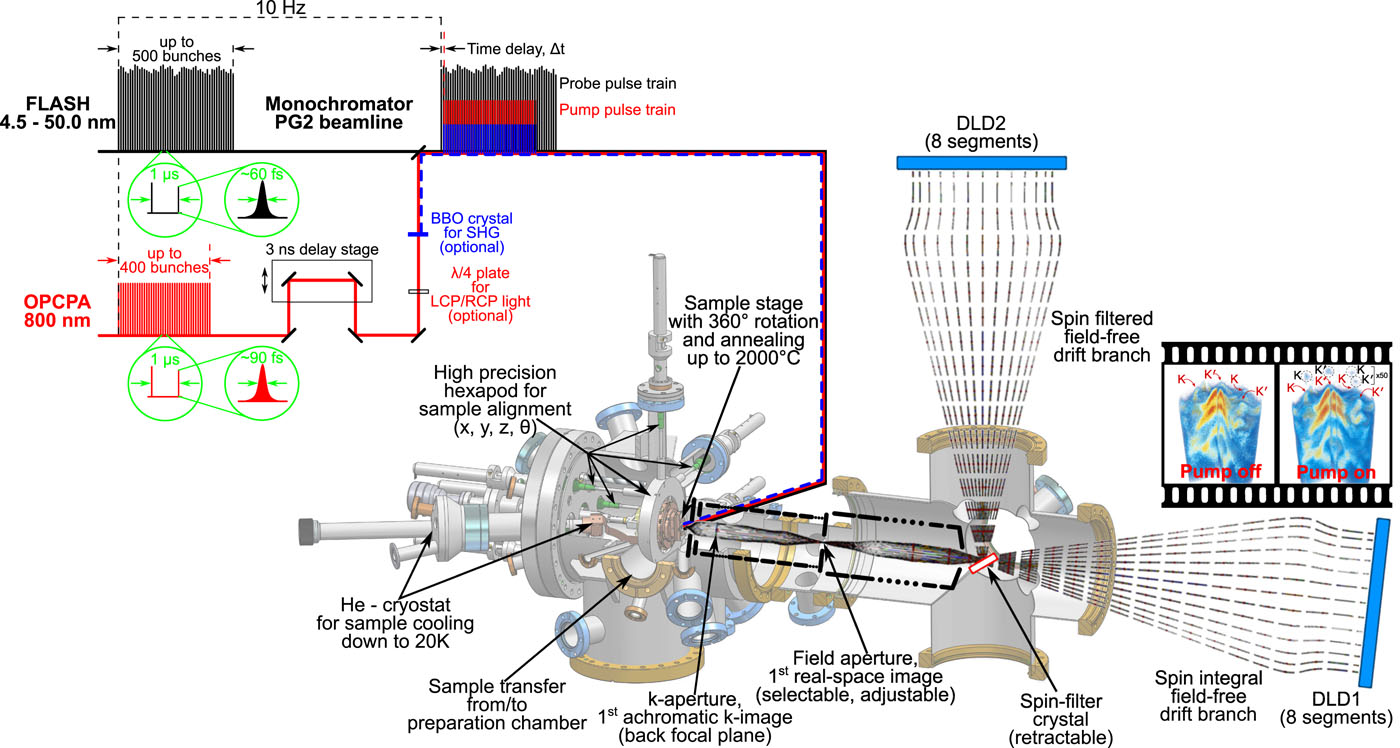
\includegraphics[width=1\linewidth]{images/2024-08-27-10-50-01.png}
    \caption{HEXTOF taken from \cite{kutnyakhovTimeMomentumresolvedPhotoemission2020}}
    % \label{fig:enter-label}
\end{figure}

\subsection{Delay Line Detectors}
The 3D detection scheme used in the \gls{HEXTOF} instrument consists of a \gls{DLD} and a \gls{TOF} tube. The \gls{DLD} is made of a \gls{MCP} for electron amplification and meanders to 

A Delayline Detector (DLD) operates by using a serpentine wire arrangement (meanders) positioned behind a micro-channel plate (MCP) for electron amplification. When particles (photons, ions, electrons) hit the MCP, they generate an electron cloud that induces electrical pulses in the meanders, allowing for precise time measurement of the hit position. This enables the reconstruction of the impact location and provides absolute time measurements relative to an external clock signal, processed by fast electronics and a time-to-digital converter (TDC).

\begin{figure}
    \centering
    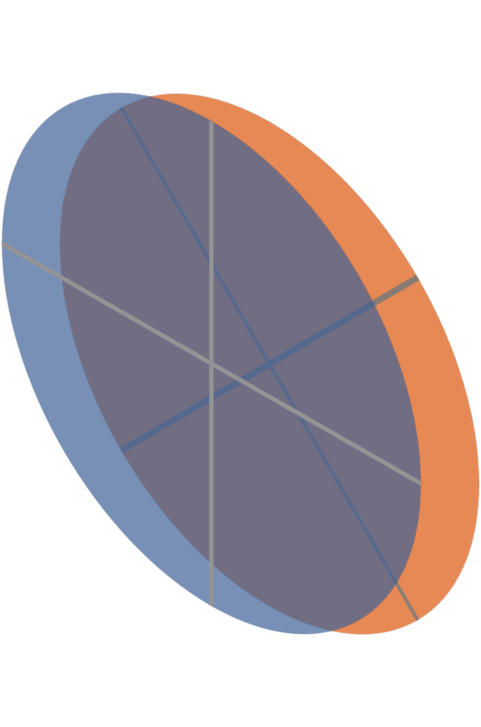
\includegraphics[width=0.3\linewidth]{images/sectors_figure.pdf}
    \caption{Schematic of the 2-layered DLD. The detector is divided into 2 layers, each with 4 sectors.}
    \label{fig:sectors}
\end{figure}

%images/chessy_deblurring_merged_events.png
\begin{figure}
    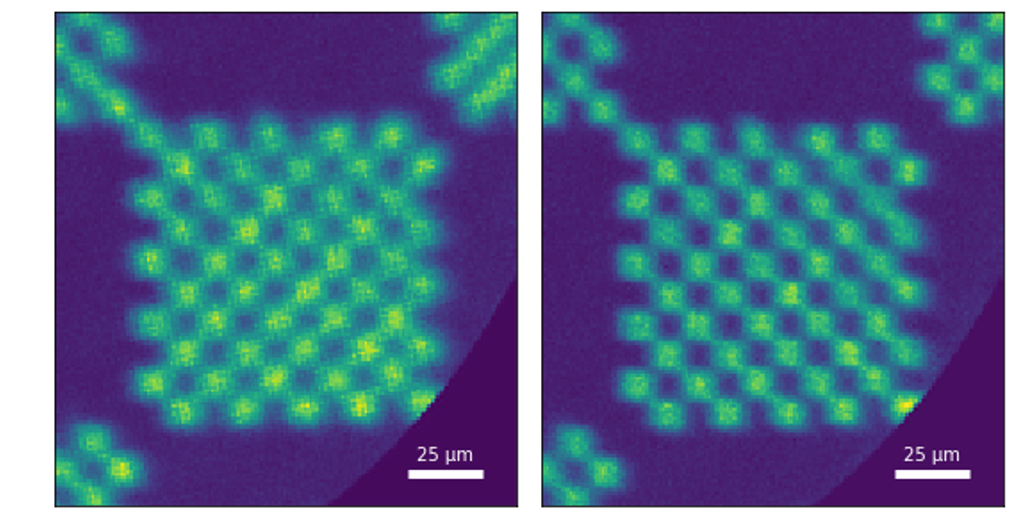
\includegraphics[width=1\linewidth]{images/chessy_deblurring_merged_events.png}
\end{figure}

\section{Binning as means of Imaging}
digital imaging from lecture
sampling etc
Binning is a way to find underlying distribution.

\section{Experimental Datasets}\label{section:datasets}
We look at four materials that have been studied using \gls{HEXTOF} at \gls{FLASH}: \gls{GrIr}, \gls{NiW}, \gls{GdW}, and \gls{WSe2}. Long acquisition times are necessary to get interpretable results. This is due to three main reasons. As mentioned above, the intrinsic stochastic nature of the photoemission process requires us to collect a large number of events to approach the true value (expected value). Additionally, the low repetition rate of the \gls{FEL} means that we need to collect data over a long period of time to get enough events. Lastly, the multidimensional acquisition scheme to simultaneously resolve \gls{kx}, \gls{ky}, \gls{kz}, \gls{E}, \gls{tpp}, and \gls{Sz} suffers from the curse of dimensionality. With an increase in dimension, the space becomes sparser, and exponentially more data is needed to fill the space.

\begin{figure}
    \centering
    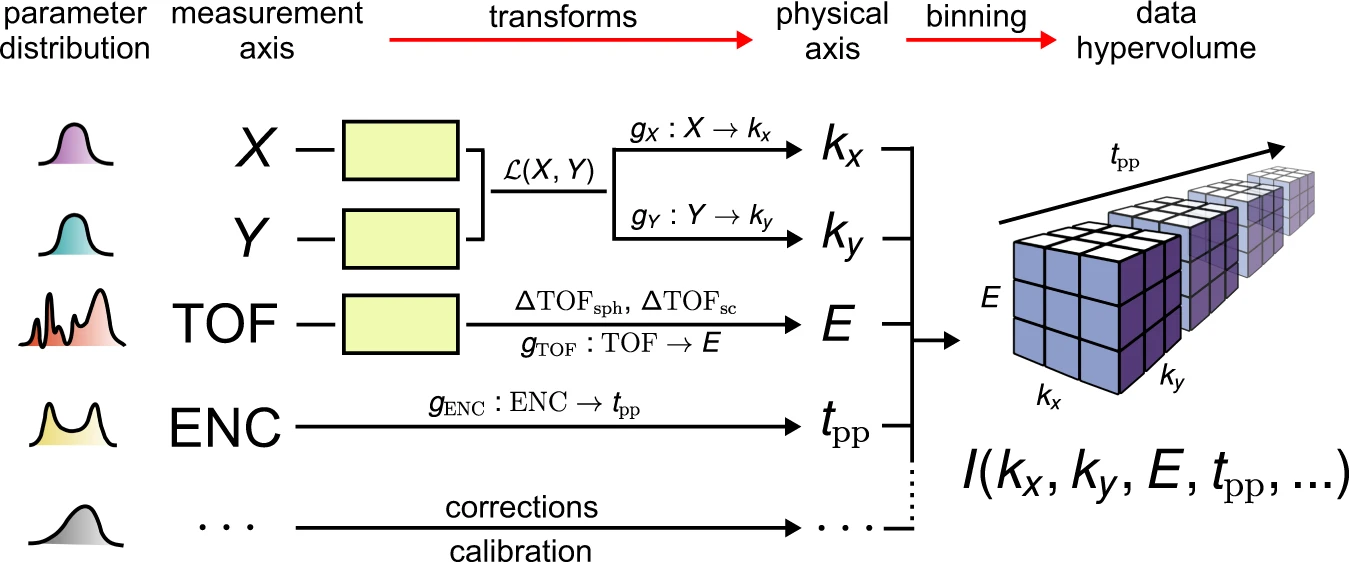
\includegraphics[width=1\linewidth]{images/2024-08-25-22-36-44.png}
    \caption{MPES taken from \cite{xianOpensourceEndtoendWorkflow2020}}
    \label{fig:mpes workflow}
\end{figure}

A 3D image is formed by binning across the three physical axes--\gls{kx}, \gls{ky} and \gls{E}--from different datasets such as the \gls{GrIr} dataset, containing \num{1.86e8} electron counts in the entire dataset. The average count decreases when binning across additional dimensions, such as the pump-probe time \gls{tpp} or spin polarization \gls{Sz}. After focusing on a \gls{ROI} (\gls{EF} and near), and binning in 3D, the total counts become \num{1.15e8}, with an average count of $\approx$1.05 per voxel. 



\begin{table}
    \centering
    \resizebox{0.6\textwidth}{!}
    {%
    \begin{tabular}{lrr}
        \toprule
         & Counts & Average Counts Per Voxel \\
         &  &  \\
        \midrule
        Noisy & \num{1e6} & 0.006 \\
        Noisy & \num{2e6} & 0.011 \\
        Noisy & \num{4e6} & 0.023 \\
        Noisy & \num{8e6} & 0.046 \\
        Noisy & \num{1.6e7} & 0.091 \\
        Noisy & \num{3.2e7} & 0.183 \\
        Noisy & \num{4.8e7} & 0.274 \\
        Noisy & \num{9.6e7} & 0.546 \\
        Target & \num{1.86e8} & 1.055 \\
        \bottomrule
    \end{tabular}
    }
\caption{Noisy realizations generated from varying total counts. The acquisition time is proportional to the total counts, with the \num{1.86e8} count dataset serving as the target.}
\label{noisy-dataset-table}
\end{table}

With the \gls{DLD} providing a stream of single-event data, we are uniquely positioned to access true noisy realizations by taking subsets of varying total electron counts from the full dataset. These subsets can then be binned to form independent 3D images.

\begin{figure}
    \centering
    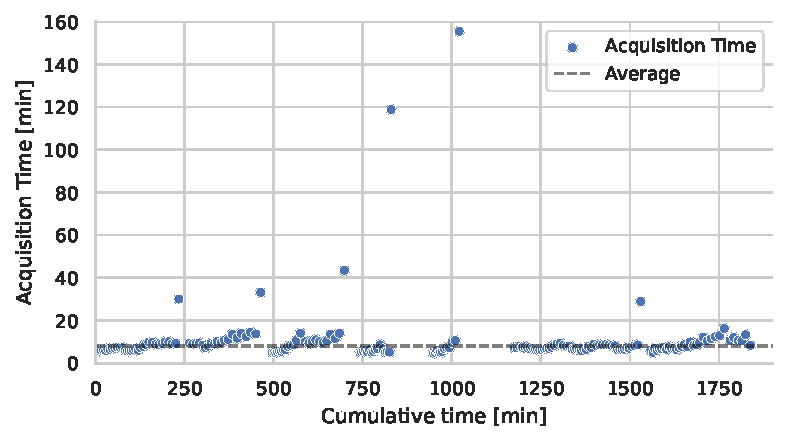
\includegraphics[width=0.8\linewidth]{images/acq_time_1M.pdf}
    \caption{Total acquisition time in minutes for generating \num{e6} data points. Some outliers are present due to the photon source being off, leading to longer acquisition times. The average acquisition time without outliers is approximately 8 minutes (see dashed line).}
    \label{fig:acq-time-1M}
\end{figure}


As seen in Figure~\ref{fig:acq-time-1M}, \num{e6} counts roughly correspond to \qty{8}{\min} of data acquisition, illustrating the total acquisition time to generate \num{e6} electron events. From the complete dataset, \texttt{186} subsets—sampled at one-million-count intervals—can be extracted. In theory, the data generation is an independent stochastic process, allowing for a large variety of randomly sampled subsets. However, in our case, the \gls{FEL} light source introduces a degree of dependence as it is not stable over extended periods, beyond its intrinsic fluctuations.

Noisy realizations can then be formed based on a number of total counts. The total counts and average counts per voxel for each noisy realization are shown in Table \ref{noisy-dataset-table}. These realizations can help evaluate the performance of denoising algorithms as a function of acquisition time. Lower count realizations ($<$e7), corresponding to shorter acquisition times, are of most interest to denoise. Successful denoising of such data could significantly improve experimental efficiency, allowing the investigators to steer the experiment in the right direction, crucial in time-limited \glspl{beamtime}. Hence, the realizations are sampled at count values: \numlist{1e6;2e6;4e6;8e6;1.6e7;3.2e7;4.8e7;9.6e7}.


\subsection{Calibration}
We present an example calibration workflow to calibrate--mapping of pixel values to the momentum axes of \gls{GrIr} dataset. Graphene is a 2D material with carbon atoms arranged in a hexagonal honeycomb structure. The Brillouin zone exhibits high-symmetry points in the reciprocal lattice (momentum space) such as the $K$-point and $K'$-point, located at the corners of the hexagonal zone, and $\Gamma$-point, located at the center \cite{castronetoElectronicPropertiesGraphene2009}. The calibration process is to map the detector pixel axes to the physical momentum axes.

In graphene's reciprocal lattice, the momentum space coordinates of the $K$-point can be derived from the lattice vectors. The reciprocal lattice vector components in the hexagonal Brillouin zone are given by:
\begin{equation*}
    k_x = \frac{2\pi}{3a}
\end{equation*}
\begin{equation*}
    k_y = \frac{2\pi}{3\sqrt{3}a}
\end{equation*}
with $a\approx$\qty{1.42}{\angstrom}, the carbon-carbon bond length. The distance from the $\Gamma$-point to $K$-point in is just:

\begin{equation*}
    d_{\Gamma K} = \sqrt{k_x^2 + k_y^2}
\end{equation*}

Substituting $a$, we obtain $d_{\Gamma K} = \qty{1.71}{\angstrom^{-1}}$. The pixel distance between the $\Gamma$-point and $K$-point in the detector image is computed to be $190$px (see Figure~\ref{fig:original-pixel-gamma-k} left). $d_{\Gamma K}/190$ then gives the scaling factor to calibrate the \gls{DLD} X and Y coordinates to \gls{kx} and \gls{ky}, respectively.
, used as a scaling factor to calibrate the momentum axes, as shown in Figure~\ref{fig:calibrated-momentum}.



\begin{figure}[ht]
    \centering
    % First subfigure (Original Image with Γ and K Points)
    \begin{subfigure}[t]{0.49\linewidth}
        \centering
        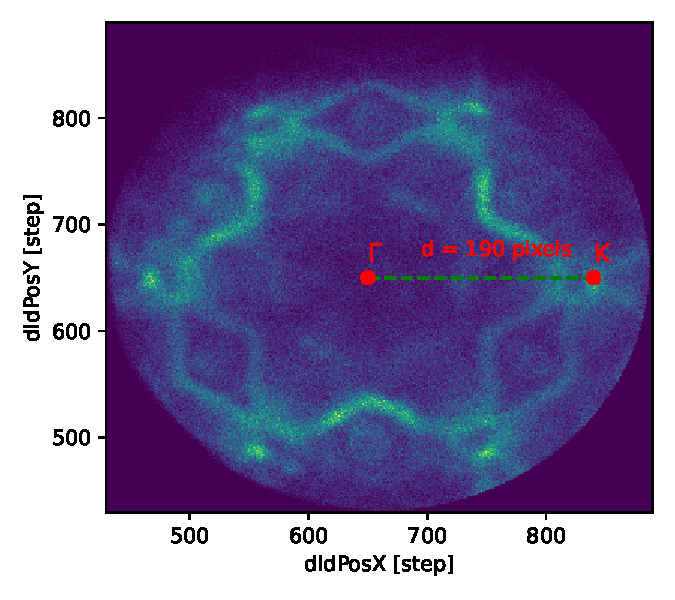
\includegraphics[width=\linewidth]{images/original_image_gamma_k.pdf}
        \caption{Uncalibrated image with \gls{DLD} X and Y coordinates, marked with the $\Gamma$ and $K$ points, and the distance between them--$190$px.}
        \label{fig:original-pixel-gamma-k}
    \end{subfigure}
    \hfill
    % Second subfigure (Momentum-Calibrated Image)
    \begin{subfigure}[t]{0.49\linewidth}
        \centering
        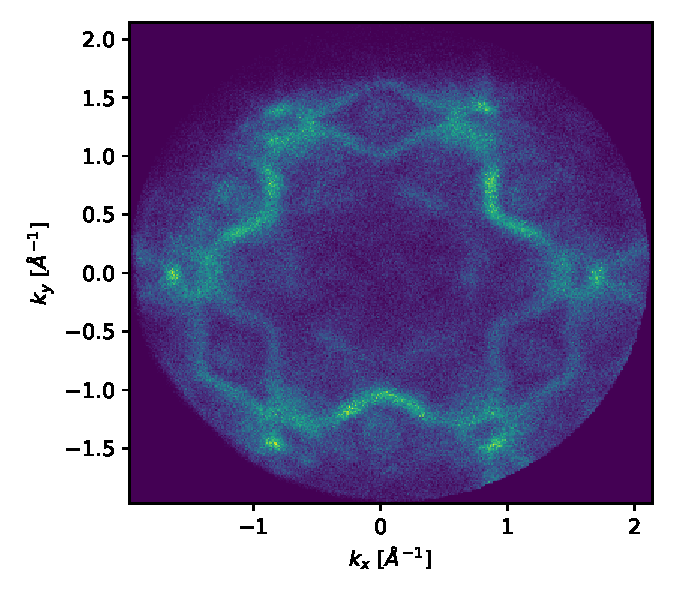
\includegraphics[width=\linewidth]{images/calibrated_momentum.pdf}
        \caption{Calibrated momentum axes.}
        \label{fig:calibrated-momentum}
    \end{subfigure}
    \caption{The detector axis and calibrated momentum axis. The left image shows the original image with the $\Gamma$ and $K$ points marked. The right image shows the calibrated momentum axes.}
\end{figure}